\documentclass{article}

\usepackage[a4paper, total={6.5in, 11in}]{geometry}

\usepackage{graphicx}
\graphicspath{{titech/ART.T458.AdvancedMachineLearning/Final2/}}

\usepackage[%
    colorlinks=true,
    pdfborder={0 0 0},
    linkcolor=red
]{hyperref}

\usepackage{latex/common}

\title{Final Report}
\date{2021 August}
\author{Sixue Wang 21M30927\\Tokyo Institute of Technology}

\begin{document}

\maketitle

\section*{Q1}
The sigmoid function is neither convex nor concave, so I would like to use gradient descent to find the optimal value. The loss function of this problem is $||f(x)-g(x)||$. In order to ensure that the optimal $b$ satisfies the constraints in the domain of $f$, I constructed the following dataset:
\begin{CMath}
  X = \{-1.0, -0.9, -0.9, ..., 0.0, 0.1, 0.2, ..., 1.0, 1.1, 1.2, ..., 2.0, 2.1, 2.2, ..., 3.0, 3.1, 3.2, ..., 4.0\} \\
  Y = \{0.0, 0.0, 0.0, ..., 2.0, 2.0, 2.0, ..., -1.0, -1.0, -1.0, ..., 3.0, 3.0, 3.0, ..., 0.0, 0.0, 0.0, ..., 0.0\}
\end{CMath}
I also need to carefully set the initial value of $b$, because $w$ has a huge magnitude and sigmoid is insensitive in that domain which means the wrong initialization will lead gradient vanish or explosion then fail to converge. So I have to give a rough solution and let gradient descent to fine-tune it.
\begin{center}
  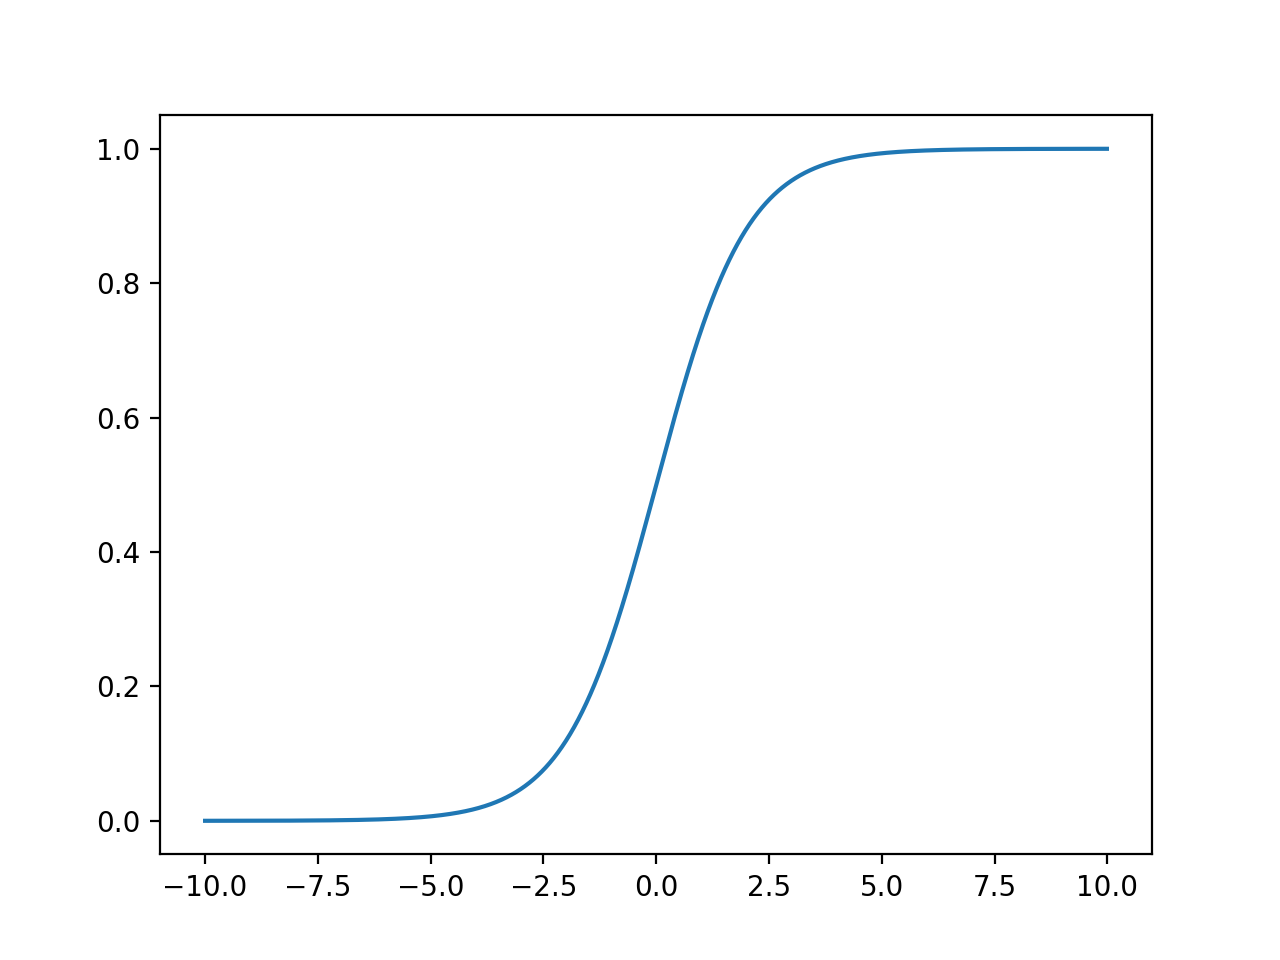
\includegraphics[scale=0.3]{sigmoid}
  \captionof{figure}{sigmoid}
\end{center}
The interesting thing is that $v = [2, -2, -1, 1, 3, -3]$, we can get one possible initialization by solving the following equations:
\begin{CMath}
  \sigma(w_0 * 0 + b_0) \approx 1 \\
  \sigma(w_1 * 1 + b_1) \approx 1 \\
  \sigma(w_2 * 1 + b_2) \approx 1 \\
  \sigma(w_3 * 2 + b_3) \approx 1 \\
  \sigma(w_4 * 2 + b_4) \approx 1 \\
  \sigma(w_5 * 3 + b_5) \approx 1 \\
\end{CMath}
where $b_i$ is decreasing. As $x$ increases, the previous $g_i$ will be offset by the new $g_i$, and the following $g_i$ will always remain 0. In my experiment, I set $b = [5, -995, -995, -1995, -1995, -2995]$ and $\epsilon=1e-4$, the optimal $b=[11.6939,  -988.3085,  -989.0007, -1989.0112, -1987.9169, -2987.8752]$.
\begin{center}
  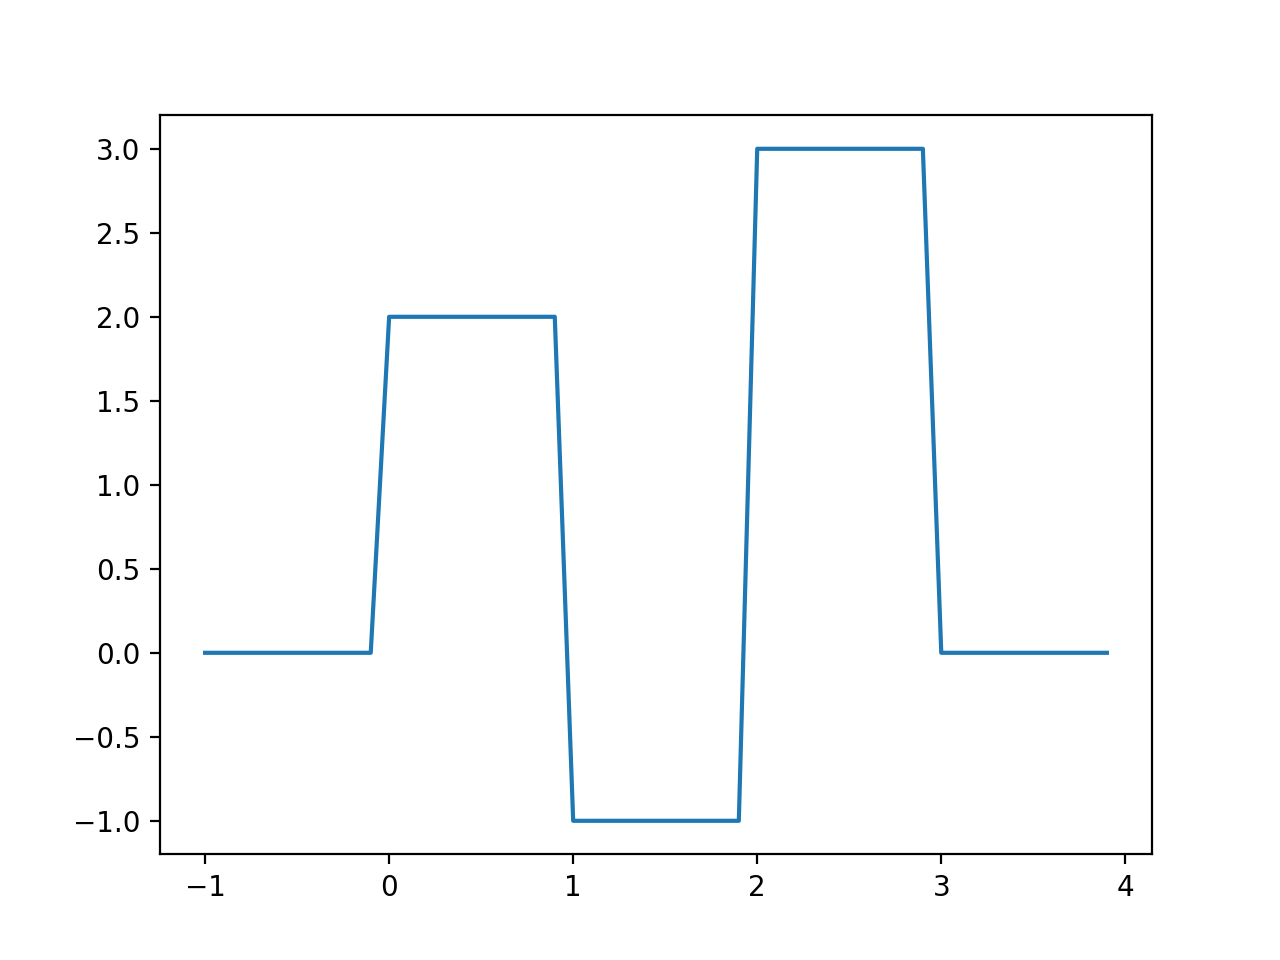
\includegraphics[scale=0.3]{q1}
  \captionof{figure}{g(x)}
\end{center}
\begin{PYCode}[q1 in pytorch]
w = torch.tensor([[1000. for _ in range(6)]])
v = torch.tensor([[2.], [-2.], [-1.], [1.], [3.], [-3.]])
b = [[5., -995., -995., -1995.0, -1995.0, -2995.0]]
b = torch.tensor(b, requires_grad=True)
f = lambda x: torch.sigmoid(x @ w + b) @ v

x = []
y = []
data = [[-1, 0, 0.], [0, 1, 2.], [1, 2, -1.], [2, 3, 3.], [3, 4, 0.]]
for l, r, val in data:
    x += [i for i in np.arange(l, r, 0.1)]
    y += [val for i in range(int((r - l) / 0.1))]
x = torch.tensor(x, dtype=torch.float32).reshape(len(x), 1)
y = torch.tensor(y).reshape(len(y), 1)

for i in range(1000000):
    loss = torch.norm(f(x) - y, p=1)
    loss.backward()
    if loss <= 1e-4:
        break
    with torch.no_grad():
        b -= 10 * b.grad
        b.grad.zero_()
\end{PYCode}

\section*{Q2}
\subsection*{(1)}
\begin{CMath}
  h       & = [0.0, 1.5] \\
  \hat{y} & = [0.5]
\end{CMath}
\subsection*{(2)}
The cross-entropy loss is used to train classification model. In our setting, $y \in R$, so I assume that $\hat{y}$ represents the positive probability, and the negative probability is $1-\hat{y}$. Now the cross-entropy loss is
\begin{CMath}
  -\hat{y} + log(exp(\hat{y})+exp(1-\hat{y}))
\end{CMath}
\begin{CMath}
  loss &= 0.6931 \\
  \frac{\partial loss}{\partial w} &= [[-0.25,-0.25],[0.0,0.0]] \\
  \frac{\partial loss}{\partial b} &= [-0.25, 0.0] \\
  \frac{\partial loss}{\partial q} &= [-0.375, 0.0] \\
  \frac{\partial loss}{\partial c} &= [-0.25] \\
\end{CMath}
\begin{PYCode}[q2 in pytorch]
w = torch.tensor([[1., 1.], [-1., -1.]], requires_grad=True)
b = torch.tensor([-0.5, 1.5], requires_grad=True)
q = torch.tensor([1., 1.], requires_grad=True)
c = torch.tensor([-1.5], requires_grad=True)
h = lambda x: torch.nn.ReLU()(w @ x + b)
y = lambda x: torch.nn.Sigmoid()(h(x).T @ q + c)

x = torch.tensor([0., 0.])
print("h = {}".format(h(x)))
print("y = {}".format(y(x)))

x = torch.tensor([1., 1.])
loss = -y(x) + torch.log(torch.exp(y(x)) + torch.exp(1.0 - y(x)))
loss.backward()
print("loss = {}".format(loss))
print("gw = {}".format(w.grad))
print("gb = {}".format(b.grad))
print("gq = {}".format(q.grad))
print("gc = {}".format(c.grad))
\end{PYCode}

\end{document}
